\chapter{Expérimentation}\label{ch:experimentation}

	La partie expérimentation de notre projet concerne principalement le test de la qualité de service (QoS). Néanmoins, nous avons dû apprendre à utiliser le routeur et à le configurer avant de pouvoir réaliser nos tests. 

\section{Connexion au routeur}

	Pour configurer le réseau nous avons dû nous connecter au routeur via l'utilitaire Putty par le port serial<->USB. De cette manière, on accède à l'interface de configuration Cisco en ligne de commande.

            \begin{figure}[h]
            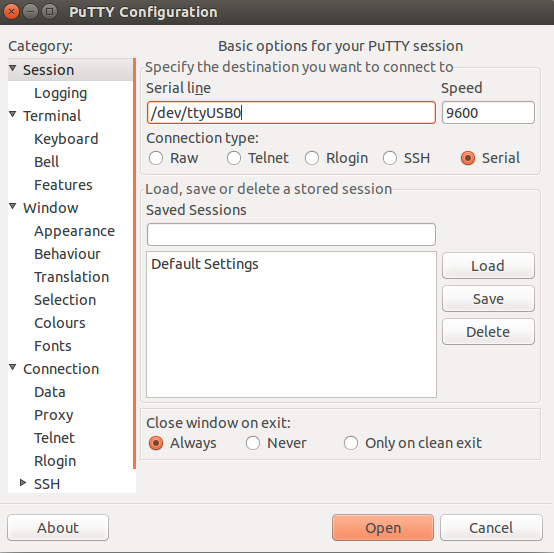
\includegraphics[width=250px]{figures/putty.png}
            \centering
            \caption{Connexion de notre ordinateur au routeur}
            \end{figure}
           
\section{Configuration du routeur}
    
	\subsection{Configuration du vlan}
    
    	Avant de connecter nos machines, il faut créer un vlan (Virtual Local Area Network) pour pouvoir utiliser IPv6. En effet, il est impossible d'activer directement l'IPv6 sur les interfaces FastEthernet 1 à 7 avec le modèle de routeur dont nous disposons.
        
    	On crée ici un vlan appelé "vlan 2" :
        \begin{lstlisting}[frame=single]
              vlan database
              vlan 2
        \end{lstlisting}
\newpage
	\subsection{Configuration des interfaces}
        	
		On configure ensuite les différentes interfaces du routeur que l'on va utiliser (fastEthernet 1 à 3 pour notre expérimentation). 
    
Exemple de la configuration de l'interface 1 :
        \begin{lstlisting}[frame=single]
            interface FastEthernet 1
            switchport mode access
            switchport access vlan 2
        \end{lstlisting}
    
    On précise que l'interface est prête à recevoir des informations avec "mode access" et qu'elle est liée au vlan 2.
    
	\subsection{Configuration IPv6}
        
        On passe en mode configuration pour l'interface du vlan 2 et on lui attribue une adresse IPv6. 
        
        On affecte à chaque machine du vlan 2 une adresse générée à partir du préfixe 2001:DB8:0:1::/64 et de l'adresse MAC de la machine (option eui-64).
        
        Configuration :
        \begin{lstlisting}[frame=single]
          interface vlan 2
          ipv6 address 2001:DB8:0:1::/64 eui-64
          ipv6 enable
          no ip address
          exit
          ipv6 unicast-routing 
        \end{lstlisting}
        
        À noter que l'on a désactivé l'adressage IPv4 avec la commande suivante afin d'être certain que nos services utilisent l'IPv6 :
        \begin{lstlisting}[frame=single]
			no ip address
        \end{lstlisting}
        
	\subsection{Test de la connexion et adressage IPv6}
        
        Une fois que la configuration IPv6 est effectuée, on connecte nos ordinateurs sur les interfaces puis on teste la connexion.
        
        Tout d'abord on vérifie qu'une adresse IPv6 a été affectée à chaque machine connectée au routeur.
Pour cela on utilise la commande suivante :

        \begin{lstlisting}[frame=single]
			ifconfig
        \end{lstlisting}
        
        \begin{figure}[h]
        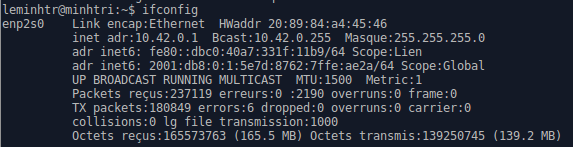
\includegraphics[width=250px]{figures/ipv6-adr.png}
        \centering
        \caption{Résultat de la commande ifconfig}
        \end{figure}
        
        On peut voir une adresse IPv6 link-local en FE80:, qui a été automatiquement affectée à la machine par défaut.
        On a également l'adresse unicast global commençant par 2001:DB8:0:1 (préfixe) suivi d'une adresse dérivée de l'adresse MAC de la machine.
        
        L'adresse multicast FF02::1 est aussi disponible par défaut, toutes les machines du LAN écoutent à cette adresse.
        L'adresse FF02::2 désigne quant à elle tous les routeurs du LAN.
        
         On teste également la connexion entre le routeur et l'ordinateur en effectuant un ping (requête ICMP echo).
            \begin{figure}[h]
            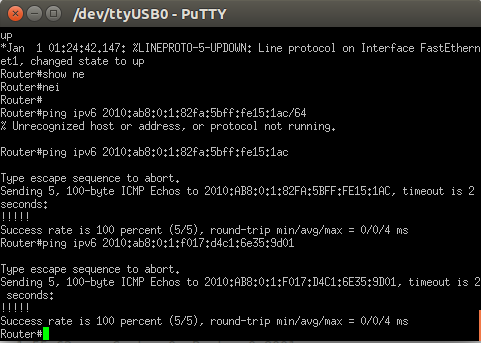
\includegraphics[width=250px]{figures/pings2.png}
            \centering
            \caption{On ping la machine depuis le routeur}
            \end{figure}

            \begin{figure}[h]
            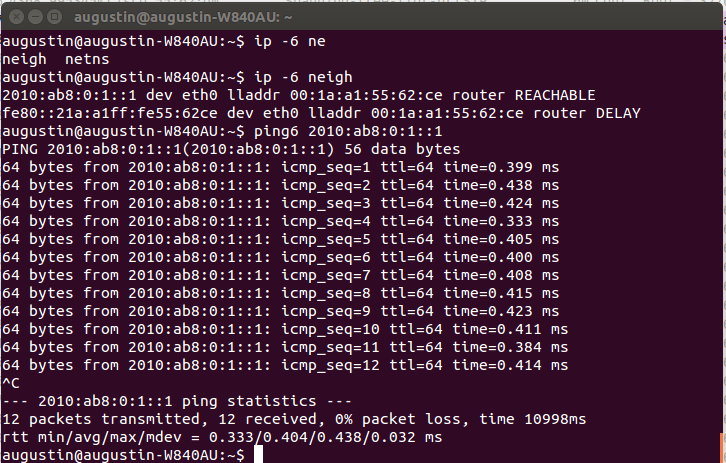
\includegraphics[width=250px]{figures/pings.png}
            \centering
            \caption{Ping depuis la machine vers le routeur}
            \end{figure}
        
    La connexion fonctionne correctement car aucun paquet n'est perdu !
    
    On peut également tester un ping sur l'adresse multicast FF02::1, en précisant l'interface de sortie, de cette manière dans un terminal :
    	\begin{lstlisting}[frame=single]
ping6 -I eth0 FF02::1
        \end{lstlisting}
     Cela permet de connaître tous les clients connectés au routeur.
    
	\subsection{Sauvegarde des différentes configurations du routeur}
    
    \subsubsection{Problème avec le chargement de le configuration de démarrage}
    
    	Nous avons rencontré un problème avec le chargement de la startup-config lorsqu'on démarre notre routeur. En effet, le mode de paramétrage du routeur faisait qu'au démarrage, la configuration n'était pas chargée depuis startup config. Nous avons donc corrigé ce problème de la manière suivante. 
    
Le paramètre de configuration registre est un code hexadécimal qui permet de changer le comportement du routeur au démarrage.\cite{config-register} Notamment : 
\begin{itemize}
\item comment le routeur démarre (ROMmon, NetBoot)
\item avec quelles options (ignorer la configuration de démarrage, désactiver les messages de démarrage)
\item la vitesse de la console (en bauds)
\end{itemize}
        
La commande :         
		\begin{lstlisting}[frame=single]
          show version
        \end{lstlisting}
permet de connaître le code du paramètre de configuration registre (dernière ligne du résultat).

Le code de paramètre de configuration registre présent à l'origine était le 0x2142 qui configure le routeur pour ignorer la configuration de démarrage (startup-config). 
Nous avons redéfini le code de paramètre de configuration registre à sa valeur par défaut sortie d'usine : 0x2102, ce qui permet de charger la configuration de démarrage au démarrage.
        
        \begin{lstlisting}[frame=single]
          show version
          conf t
          config-register 0x2102
        \end{lstlisting}
        
	    \begin{figure}[h]
        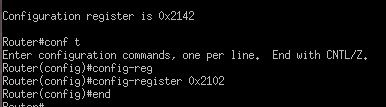
\includegraphics[width=250px]{figures/config-register_0x2102.png}
        \centering
        \caption{Modification du paramètre de configuration}
        \end{figure}

	\subsubsection{Sauvegardes et changements de configurations}

		Nous avons sauvegardé différentes configurations du routeur (avec et sans QoS) dans des fichiers sur la carte compact flash du routeur, par exemple dans le fichier SR04QOS : 
        \begin{lstlisting}[frame=single]
          copy running-config SR04QOS
        \end{lstlisting}
        
        Pour changer de configuration (passer d'une configuration sans QoS à une configuration avec QoS par exemple), on copie le fichier de configuration de la carte dans la startup-config puis on recharge la configuration du routeur :
        
        \begin{lstlisting}[frame=single]
            copy SR04QOS startup-config
            reload
        \end{lstlisting}


    \section{Mise en place des services}
    
    Pour tester la qualité de service, nous avons mis en place quelques services pour tester la connexion. Nous nous sommes concentrés sur les logiciels de voix sur IP puis par la suite, nous avons fait du streaming vidéo. 
    
    Note : Les services ont été mis en place sur un ordinateur utilisant ArchLinux (gestion de service : systemctl). Les configurations des serveurs et les procédures d'installation ne sont pas présentées ici car hors-sujet.
    
	\subsection{Conférence audio}
    
    	Nous avons installé et hébergé un serveur Murmur sur une de nos machines. Murmur permet d'héberger des salons de discussions (conversation vocale et écrite) du logiciel Mumble. Mumble est un logiciel permettant la voix sur IP, et permet donc de communiquer oralement à distance. 

Il faut d'abord se connecter au serveur Murmur que nous avons créé. L'adresse est l'adresse IPv6 de l'ordinateur faisant tourner le serveur.
        \begin{figure}[h]
        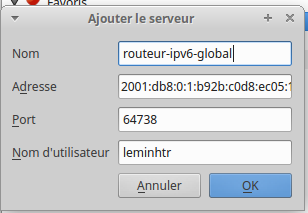
\includegraphics[width=250px]{figures/mumble-config.png}
        \centering
        \caption{Connexion au serveur Murmur dans Mumble}
        \end{figure}
        
Il est également possible d'activer/désactiver la QoS sur Mumble, fonctionnalité utile pour nos tests.

        \begin{figure}[h]
        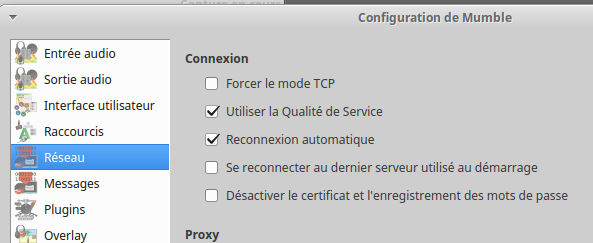
\includegraphics[width=250px]{figures/qos-mumble-config2.png}
        \centering
        \caption{Option QoS de Mumble}
        \end{figure}


Enfin, nous avons réussi à discuter par message écrit et VoIP (une bouche est rouge quand une personne parle par VoIP)

        \begin{figure}[h]
        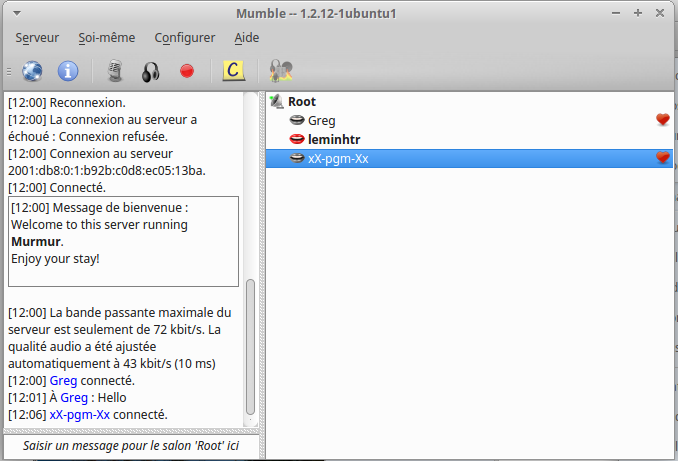
\includegraphics[width=250px]{figures/qos-mumble-talk.png}
        \centering
        \caption{Salon de discussion Mumble (3 personnes)}
        \end{figure}
        
\newpage
        
	\subsection{Transfert de fichier}
        Nous avons installé et hébergé un serveur SSH pour le transfert de fichier en SFTP (openSSH).

		\begin{figure}[!h]
          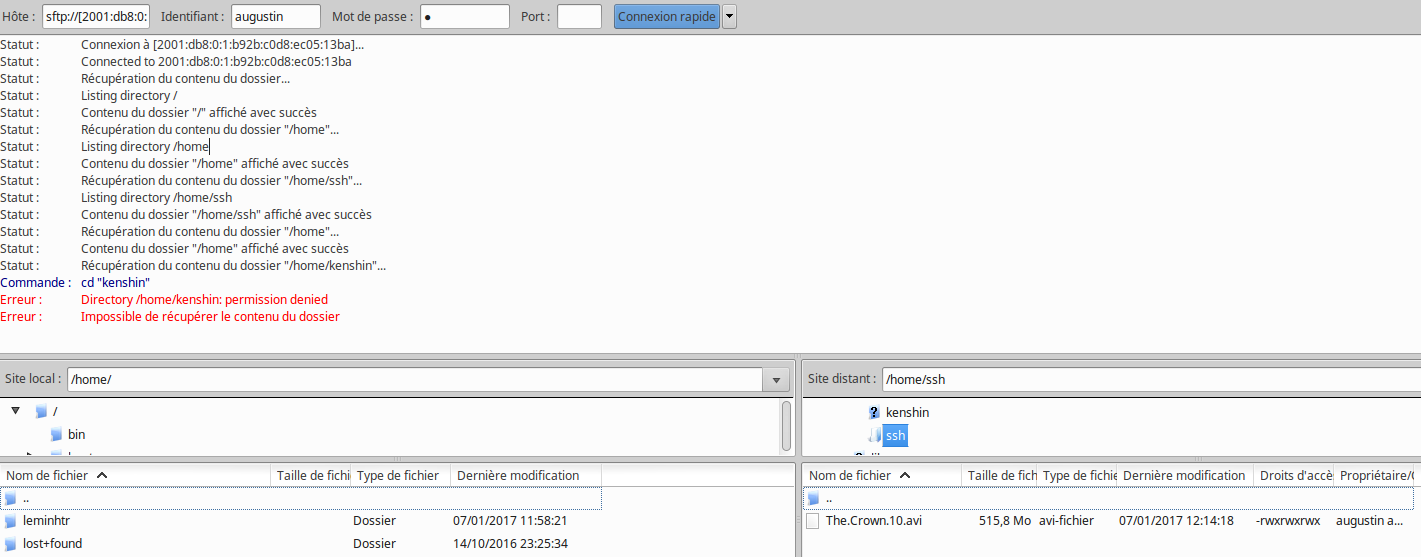
\includegraphics[width=400px]{figures/filezilla.png}
          \centering
          \caption{Configuration et accès au serveur SSH}
        \end{figure}

	\subsection{Téléphonie}
    
    Bien que nous ayons déjà pu tester la VoIP avec Mumble, nous voulions voir ce que cela donnait avec des téléphones. Nous avons donc emprunté deux téléphones utilisant la VoIP fournis par le département du GI.
    
    Le téléphone possède deux méthodes d'alimentation possible : PoE (Power over Ethernet) ou par alimentation classique (Transformateur 220v -> 36V).
    Le POE permet de transmettre à un équipement à la fois des données, mais aussi son alimentation électrique via le câble Ethernet, deux des quatre paires du câble sont allouées à l'alimentation électrique. Cette technique permet d'éviter l’installation d’un double réseau (IP et électrique). Cependant, le routeur ne dispose pas de l'option facultative permettant le support de la PoE. L'alimentation s'est donc faite via transformateur.
    
    La mise en place du téléphone fut assez longue : nous avons dû lire la documentation technique pour téléphone. La mise en place de 4 serveurs (TFTP, FTP, HTTP, SIP) ainsi qu'une configuration assez complète, notamment pour la gestion du protocole SIP. Nous avons appris par ce biais à mettre en place une architecture VOIP complète qui nous a permis de passer des appels entre tous nos différents appareils : téléphone portable (via Linphone), ordinateur (via Ekiga) et bien sûr, via le téléphone IP.
    
   
	\subsection{Vidéo à la demande, streaming}
    
    	Nous avons implémenté un serveur HTTP afin de pouvoir faire du streaming vidéo.
        \begin{lstlisting}[frame=single]
vlc -vvv '/home/ssh/film.avi' --ipv6 --sout'#
transcode{vcodec=h264,acodec=mpga,ab=128,channels=2,
samplerate=44100}:http{mux=ffmpeg{mux=flv},dst=:8080/SR04}'
--ttl 12 --sout-all 
        \end{lstlisting}
        
        \begin{figure}[!h]
        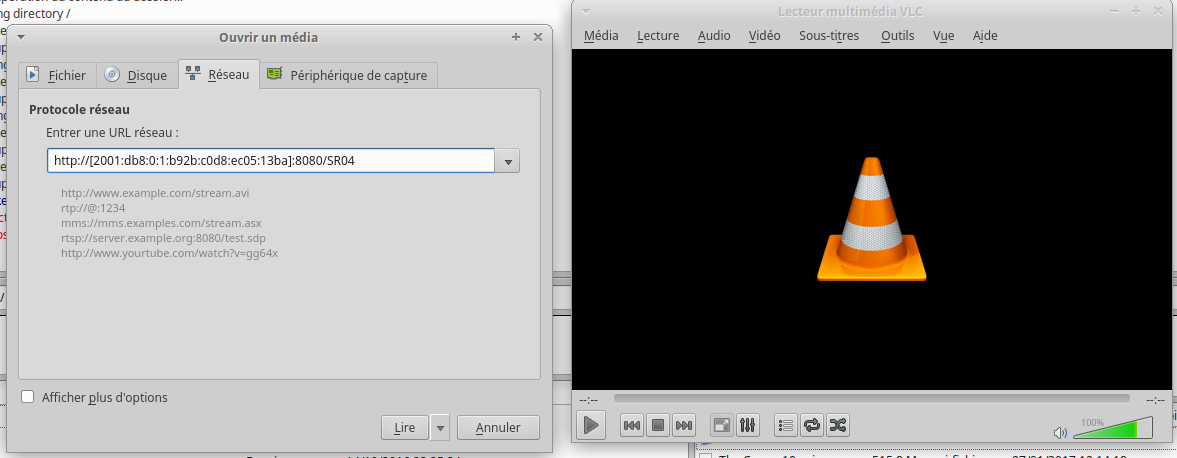
\includegraphics[width=400px]{figures/qos-vlc-config.png}
        \centering
        \caption{Configuration de l'accès au streaming}
        \end{figure}

        \begin{figure}[h]
        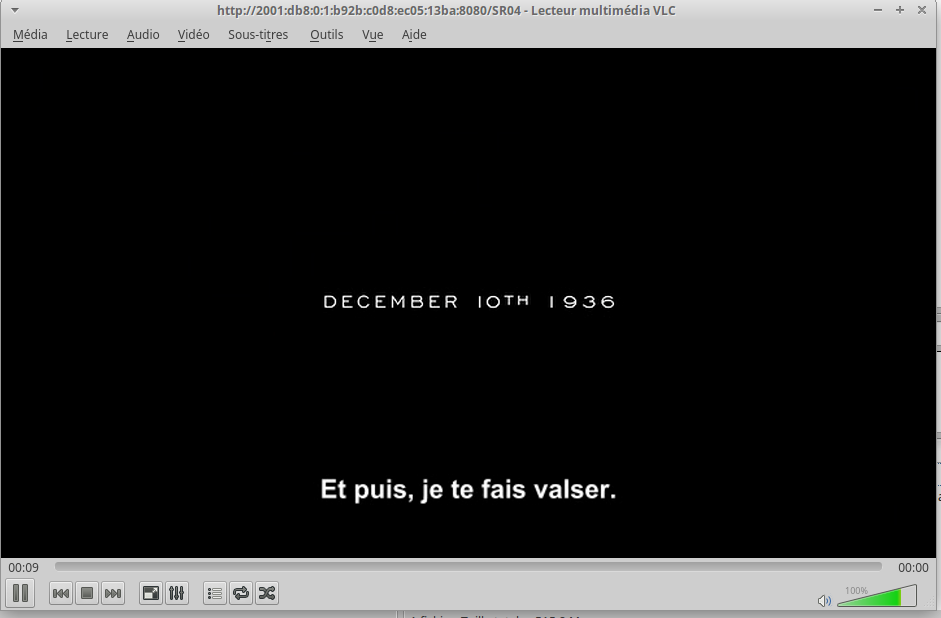
\includegraphics[width=250px]{figures/qos-vlc-stream.png}
        \centering
        \caption{Streaming d'une vidéo}
        \end{figure}

   Au cours de nos différents essais de streaming, nous avons également essayé le protocole RTP (Real-time Transport Protocol) et son homologue gérant la qualité de service : le protocole RTCP (RTP Control Protocol). RTCP sert à s'assurer de la qualité de service et permet de synchroniser les flux. Pour utiliser ces protocoles, nous avons dû créer et utiliser un groupe multicast. 
    
%%%%%%%%%%%%%%%%%%%%%%%%%%%%%%%%%%%%%%%%%%%%%%%%%%%%%%
    \section{Mise en place de la qualité de service}

		Pour mettre en place notre qualité de service, nous nous sommes basés sur les services différenciés (DS - Differentiated Services), expliqués section \ref{diffserv}. Ce type de QoS utilise le champ Traffic Class d'un paquet IPv6 afin de préciser le DSCP (Differentiated Services Code Point). Le DSCP est un code permettant de classifier et de gérer les paquets d'un réseau suivant une certaine priorité. Ainsi, on peut demander au routeur d'accélérer au maximum le passage de certains paquets en précisant le code DSCP "EF" dans leur champ Traffic Class. Cette QoS est gérée au niveau de chaque routeur, suivant leur politique de traitement des paquets. Lorsqu'aucun code DSCP n'est entré, le routeur applique une politique par défaut : "best effort".

		Ci-dessous se trouvent les instructions permettant d'implémenter la qualité de service.

		%%%%%%%%%%%%%%%%%%%%%%%%%%%%%%%%%%%%%%
		\subsection{Configuration d'une classe}
        
        Supposons que l'on veuille donner la priorité aux paquets échangés entre un serveur Http et un ordinateur, sur le port 80.
        
        En utilisant la commande ci-dessous, on crée un groupe d'accès appelé 100. Ce groupe va référencer les paquets provenant du port 80 (eq 80) de n'importe quelle source (premier any) vers n'importe quelle destination (second any). 
        \begin{lstlisting}[frame=single]
access-list 100 permit tcp any any eq 80
        \end{lstlisting}
        
        On crée ensuite une classe nommée "http". Une classe permet de représenter un ensemble de paquets sur lesquels on va appliquer une politique de traitement. La commande "match..." permet donc de spécifier les conditions d'appartenance à la classe. Ici, il faut que le paquet soit dans le groupe 100. 
        \begin{lstlisting}[frame=single]
class-map http
match access-group 100
        \end{lstlisting}
         
        %%%%%%%%%%%%%%%%%%%%%%%%%%%%%%%%%%%%%%%
        \subsection{Configuration d'une politique de traitement des paquets}

		Une fois que l'on connaît les paquets sur lesquels appliquer la QoS, il ne reste plus qu'à préciser la politique de traitement. 
        Ici, on crée une politique nommée "acceshttp" qui s'appliquera à la classe "http". On précise ensuite la priorité que l'on donne aux paquets avec "set dscp". 
		\begin{lstlisting}[frame=single]
policy-map acceshttp 
class http
set dscp cs4
        \end{lstlisting}
       
        Il ne reste plus qu'à ajouter la politique de traitement au vlan. "output" permet de préciser si le traitement se fait en entée ou en sortie du routeur. 
        \begin{lstlisting}[frame=single]
interface vlan 2 
service-policy output acceshttp
        \end{lstlisting}

		De cette manière, les paquets allant vers le port 80 auront leur champ DSCP à cs4. Ils seront prioritaires sur les autres ! Attention tout de même lorsqu'on précise un DSCP, il existe une hiérarchie entre les différents codes. Certains seront prioritaires sur d'autres.
        
        Il est possible de préciser beaucoup plus de conditions au niveau des classes. On peut conditionner les paquets suivant leur adresse IP, suivant un protocole utilisé (RTP par exemple)...
        
        De même, on peut réaliser des politiques de traitement plus poussées, en allouant par exemple un pourcentage de la bande passante aux paquets d'une classe.
        
        L'ensemble de méthode de tri (class-map) et des politiques (policy) sont disponibles ici \url{https://www.cisco.com/c/en/us/td/docs/ios/12_2/qos/configuration/guide/fqos_c/qcfmcli2.html}

%%%%%%%%%%%%%%%%%%%%%%%%%%%%%%%%%%%%%%%%%%%%%%%%%%%%%%
    \section{Test de la qualité de service}
    
    %%%%%%%%%%%%%%%%%%%%%%%%%%%%%%%%%
    \subsection{Saturation du réseau}
       
    Pour tester la QoS, nous avons cherché à saturer le réseau. Pour cela, nous avons fait du streaming d'une vidéo 1080p sur deux postes. La vidéo reçue par le poste de droite \ref{vlc-compar} a des difficultés à s'afficher en temps réel (problème de Codec, la charge sur le réseau reste la même).
		\begin{figure}[h]
        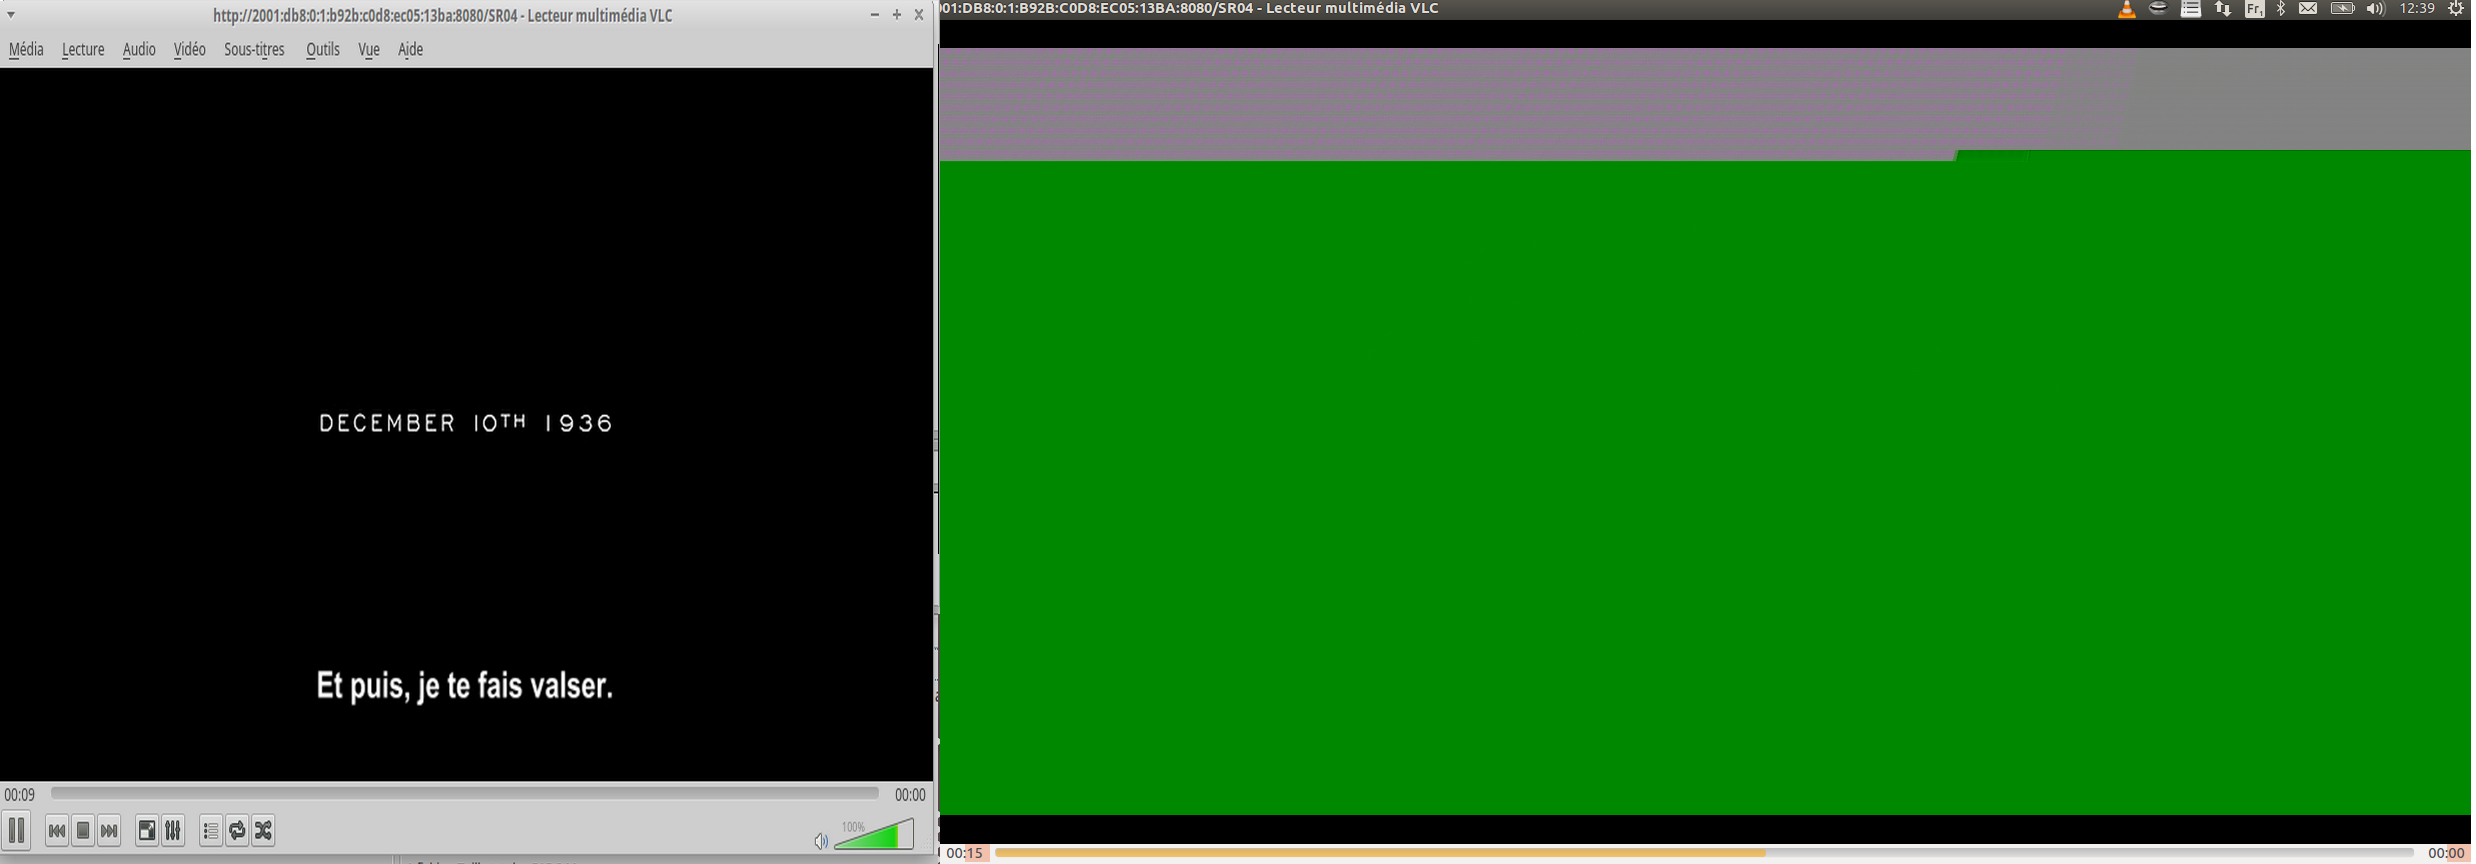
\includegraphics[width=400px]{figures/vlc-stream-compar.png}
        \centering
        \caption{Streaming d'une vidéo par 2 postes}
        \label{vlc-compar}
        \end{figure}
	
    Pendant la saturation du réseau, nous avons tenté de passer un appel VOIP sur Mumble. La latence était importante et la qualité mauvaise. Le besoin de la QoS se faisait ressentir.
      
    %%%%%%%%%%%%%%%%%%%%%%%%%%%%%%%%%%%
    \subsection{Test de la QoS par Ping}
    
    Pour prouver le bon fonctionnement de la QoS, nous avons trouvé une méthode se servant de l'utilitaire ping. Nous avons ensuite observé les paquets sur Wireshark. 
    
    La commande suivante permet d'envoyer un paquet en spécifiant le ToS(Type of Service) souhaité. Le ToS est un code comprenant le DSCP. On peut l'obtenir par la formule DSCP*4 = TOS, ou par des tables de conversion comme celle-ci : \cite{TOSDSCP}.
        \begin{lstlisting}[frame=single]
ping6 -Q <ToS> <adresse IP>
ping6 -Q 0x68 fe80::4ab9:ab2:77dd:ee4c%en3
        \end{lstlisting}  
  
    L'idée du test est donc d'activer la QoS au niveau du routeur et de charger le réseau en envoyant un fichier très lourd par exemple. On envoie ensuite un ping pour vérifier que la valeur DSCP entrée n'est pas perdue en cours de route. On peut voir cela avec Wireshark, qui repère le champ correspondant au DSCP et la priorité fixée. On peut également vérifier l'impact de la QoS entre un ping normal et un ping spécifiant le DSCP. On utilise la priorité EF, Expedited Forwarding, améliorant le temps d'acheminement du paquet.
    
        \begin{figure}[h]
        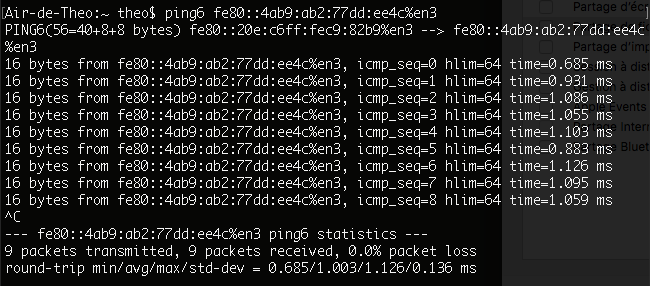
\includegraphics[width=350px]{figures/ping_sans_qos.png}
        \centering
        \caption{Envoie d'un ping sans QoS}
        \end{figure}
        
        \begin{figure}[h]
        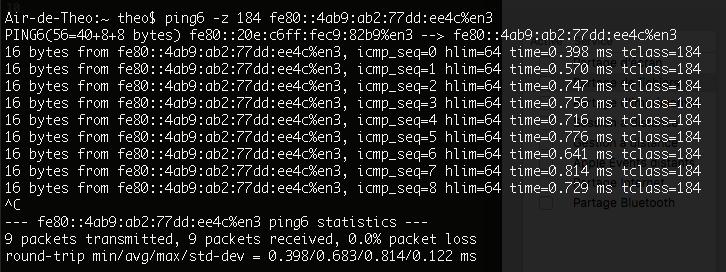
\includegraphics[width=350px]{figures/ping_qos.png}
        \centering
        \caption{Envoie d'un ping avec QoS}
        \end{figure}
        
    Petite remarque, la commande est ici ping6 -Z car elle a été réalisée sur Mac OS.
    
    En moyenne le ping met 1.003 ms pour arriver sans QoS et 0.683 ms avec QoS.
    
    Cela représente donc une amélioration de 68\% (0.683/1.003) du temps d'acheminement.
      
    On a choisi les codes DSCP correspondants au téléphone VoIP que nous avions afin de passer le Per-Hop Behavior des paquets de notre téléphone en AF, alors que tous les autres paquets étaient en default. La téléphonie VoIP devient donc prioritaire.
    
    %mettre tous les screens wireshark
    Pour le code DSCP : EF, le Per-Hop Behavior est EF (Expedited Forwarding).
    Le routeur met en priorité les ressources nécessaires pour réduire les délais, la gigue, les pertes par un service de bout en bout. Cela est très utile pour assurer le trafic temps-réel des applications telles que la VoIP ou le streaming vidéo. Il y a cependant une limite concernant le nombre de paquets marqué par un code DSCP à EF pour limiter la surcharge et les délais.
    
    Nous avons effectué un ping avec EF (Les bits DSCP sont à 46 en décimal.).
        \begin{figure}[h]
        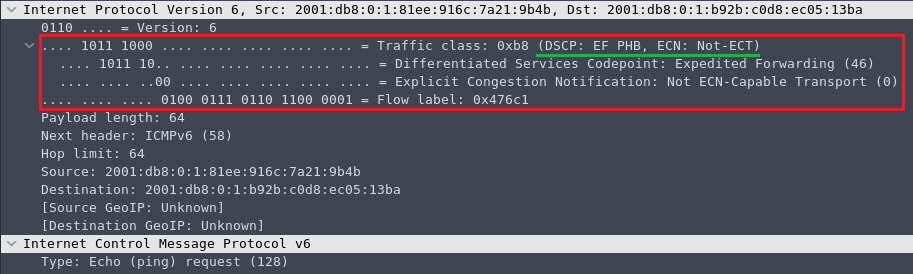
\includegraphics[width=350px]{figures/dscp-ef-color.png}
        \centering
        \caption{Expedited Forwarding PHB}
        \end{figure}
        
	Pour le code DSCP : AF31, le Per-Hop Behavior est AF (Assured Forwarding).
    Dans ce cas, l'émetteur est assuré de la réception tant que la congestion du réseau n'est pas trop significative. Une partie de la bande passante est garantie et les classes d'AF peuvent avoir accès à un supplément si possible. Il existe plusieurs classes d'AF (\ref{af_class}). Elles se distinguent par des niveaux de priorité croissant (Classe) et la probabilité de perte (Faible, moyenne, haute).
        \begin{figure}[h]
        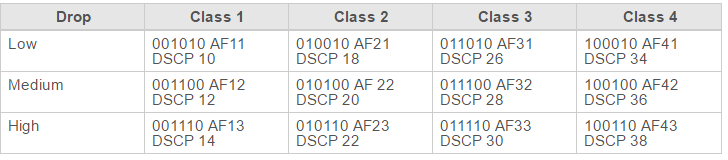
\includegraphics[width=350px]{figures/dscp_af-class.PNG}
        \centering
        \caption{Classe d'AF}
        \label{af_class}
        \end{figure}
\newpage        
        Nous avons ici effectué un ping avec AF31, cela correspond donc à une classe 3 avec une faible probabilité de perte.
        \begin{figure}[h]
        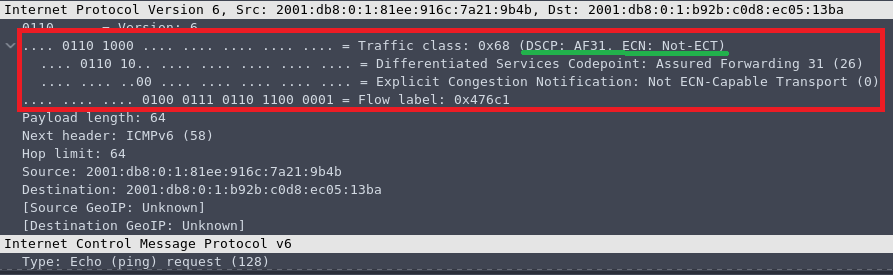
\includegraphics[width=350px]{figures/dscp-af-color.png}
        \centering
        \caption{Assured Forwarding PHB}
        \end{figure}
        
       
    Pour tous les autres codes : le Per-Hop behavior est default. Le comportement est alors \textit{"Best Effort"}.
		\begin{figure}[h]
        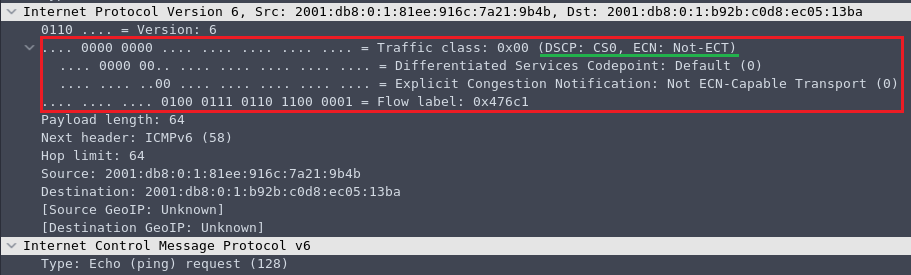
\includegraphics[width=350px]{figures/dscp-dflt-color.png}
        \centering
        \caption{Default PHB}
        \end{figure}
        
 	%%%%%%%%%%%%%%%%%%%%%%%%%%%%%%%%%%%%%%%
    \subsection{Test de la QoS par l'essai}
    
	Une fois la QoS fonctionnelle, nous avons recommencé l'expérience de départ : Streaming d'une vidéo 1080p sur deux ordinateurs. Lorsque le réseau était saturé, nous avons tenté un appel VOIP. Cette fois-ci, c'est la vidéo qui était ralentie. L'appel ne présentait aucune latence. 
    L'objectif de la QoS était atteint : c'est l'appel VOIP qui était prioritaire sur le streaming vidéo.
  	
    
    
    
    
    
    
    